%% abtex2-modelo-artigo.tex, v-1.7.1 laurocesar
%% Copyright 2012-2013 by abnTeX2 group at http://abntex2.googlecode.com/ 
%%
%% This work may be distributed and/or modified under the
%% conditions of the LaTeX Project Public License, either version 1.3
%% of this license or (at your option) any later version.
%% The latest version of this license is in
%%   http://www.latex-project.org/lppl.txt
%% and version 1.3 or later is part of all distributions of LaTeX
%% version 2005/12/01 or later.
%%
%% This work has the LPPL maintenance status `maintained'.
%% 
%% The Current Maintainer of this work is the abnTeX2 team, led
%% by Lauro César Araujo. Further information are available on 
%% http://abntex2.googlecode.com/
%%
%% This work consists of the files abntex2-modelo-artigo.tex and
%% abntex2-modelo-references.bib
%%

% ------------------------------------------------------------------------
% ------------------------------------------------------------------------
% abnTeX2: Modelo de Artigo Acadêmico em conformidade com
% ABNT NBR 6022:2003: Informação e documentação - Artigo em publicação 
% periódica científica impressa - Apresentação
% ------------------------------------------------------------------------
% ------------------------------------------------------------------------

\documentclass[
	% -- opções da classe memoir --
	article,			% indica que é um artigo acadêmico
	11pt,				% tamanho da fonte
	oneside,			% para impressão apenas no verso. Oposto a twoside
	a4paper,			% tamanho do papel. 
	% -- opções da classe abntex2 --
	%chapter=TITLE,		% títulos de capítulos convertidos em letras maiúsculas
	%section=TITLE,		% títulos de seções convertidos em letras maiúsculas
	%subsection=TITLE,	% títulos de subseções convertidos em letras maiúsculas
	%subsubsection=TITLE % títulos de subsubseções convertidos em letras maiúsculas
	% -- opções do pacote babel --
	english,			% idioma adicional para hifenização
	english,				% o último idioma é o principal do documento
	%twocolumn,         % usa duas colunas
	]{abntex2}

% ---
% PACOTES
% ---

% ---
% Pacotes fundamentais 
% ---
\usepackage{cmap}				% Mapear caracteres especiais no PDF
\usepackage{lmodern}			% Usa a fonte Latin Modern
\usepackage[T1]{fontenc}		% Selecao de codigos de fonte.
\usepackage[utf8]{inputenc}		% Codificacao do documento (conversão automática dos acentos)
\usepackage{indentfirst}		% Indenta o primeiro parágrafo de cada seção.
\usepackage{nomencl} 			% Lista de simbolos
\usepackage{color}				% Controle das cores
\usepackage{graphicx}			% Inclusão de gráficos
\usepackage{float}
% ---
		
% ---
% Pacotes adicionais, usados apenas no âmbito do Modelo Canônico do abnteX2
% ---
\usepackage{lipsum}				% para geração de dummy text
% ---
		
% ---
% Pacotes de citações
% ---
\usepackage[english,hyperpageref]{backref}	 % Paginas com as citações na bibl
% \usepackage[alf]{abntex2cite}	% Citações padrão ABNT
% ---

% set images path
\graphicspath{ {images/} }
% ---
% Configurações do pacote backref
% Usado sem a opção hyperpageref de backref
\renewcommand{\backrefpagesname}{Page(s):~}
% Texto padrão antes do número das páginas
\renewcommand{\backref}{}
% Define os textos da citação
\renewcommand*{\backrefalt}[4]{
	\ifcase #1 %
		%
	\or
		Page: #2.%
	\else
		#1 citations on pages: #2.%
	\fi}%
% ---

% ---
% Informações de dados para CAPA e FOLHA DE ROSTO
% ---
\titulo{Conversational Task Recognition Agent}
\autor{Gilberto Ribeiro Paz da Rosa\thanks{grprosa@inf.ufrgs.br}}
\local{Brasil}
\data{2016, v1.0.0}
% ---

% ---
% Configurações de aparência do PDF final

% alterando o aspecto da cor azul
\definecolor{blue}{RGB}{41,5,195}

% informações do PDF
\makeatletter
\hypersetup{
     	%pagebackref=true,
		pdftitle={\@title}, 
		pdfauthor={\@author},
    	pdfsubject={Practical application of conversational agents},
	    pdfcreator={LaTeX with abnTeX2},
		pdfkeywords={abnt}{latex}{abntex}{abntex2}{cientific article}, 
		colorlinks=true,       		% false: boxed links; true: colored links
    	linkcolor=blue,          	% color of internal links
    	citecolor=blue,        		% color of links to bibliography
    	filecolor=magenta,      		% color of file links
		urlcolor=blue,
		bookmarksdepth=4
}
\makeatother
% --- 

% ---
% compila o indice
% ---
\makeindex
% ---

% ---
% Altera as margens padrões
% ---
\setlrmarginsandblock{4cm}{4cm}{*}
\setulmarginsandblock{4cm}{4cm}{*}
\checkandfixthelayout
% ---

% --- 
% Espaçamentos entre linhas e parágrafos 
% --- 

% O tamanho do parágrafo é dado por:
\setlength{\parindent}{1.3cm}

% Controle do espaçamento entre um parágrafo e outro:
\setlength{\parskip}{0.2cm}  % tente também \onelineskip

% Espaçamento simples
\SingleSpacing

% ----
% Início do documento
% ----
\begin{document}
\selectlanguage{english}
% Retira espaço extra obsoleto entre as frases.
\frenchspacing 

% ----------------------------------------------------------
% ELEMENTOS PRÉ-TEXTUAIS
% ----------------------------------------------------------

%---
%
% Se desejar escrever o artigo em duas colunas, descomente a linha abaixo
% e a linha com o texto ``FIM DE ARTIGO EM DUAS COLUNAS''.
% \twocolumn[    		% INICIO DE ARTIGO EM DUAS COLUNAS
%
%---
% página de titulo
\maketitle

% resumo em português
\begin{resumoumacoluna}
Conversational task recognition system is a practical application of conversational agents using a valued probabilistic transition graph.
This work makes an overview of tooling used and why, implementation details of the graph, the probabilistic model used and relevant parts
of algorithms.
 
 \vspace{\onelineskip}
 
 \noindent
 \textbf{keywords}: conversational agents, word recognition, probabilistic model.
\end{resumoumacoluna}

% ]  				% FIM DE ARTIGO EM DUAS COLUNAS
% ---

% ----------------------------------------------------------
% ELEMENTOS TEXTUAIS
% ----------------------------------------------------------
\textual

% ----------------------------------------------------------
% Introdução
% ----------------------------------------------------------
\section*{Introduction}

Conversational agents are for a long time being used for systems to build a 
humanized layer between human interaction and task execution of automated environments.
More recently, big companies are trying to reach the next level of voice interactive
services using large sets of audio and text data to process and classify user audio
inputs creating deep knowledge graphs to respond more human likely way.

This work creates a graph with it's nodes, named knots here, via probabilistic transition
threshold. Navigation on the graph can only occurs if user input matches, in percentage, at
least the minimum value of the edge. Each transition executes a predefined command and
template when entering on knot.

% ----------------------------------------------------------
% Seção de explicações
% ----------------------------------------------------------
\section{Objective}

Create a conversational agent that is capable of executing pre defined tasks throughout
voice user inputs and respond with templates texts synthesized as voice output. 

\section{Tool set}

\subsection{IBM\textregistered{}  Watson\textregistered{}}

Watson API is used sessionless for speech synthesizer text responses and speech recognizer
making the system process only text transcribed from user voice input.

\subsection{Web Technologies}

User interface and the full system was develop using front-end web technologies, since the graph
and the probabilistic linking between knots to audio recording and reproduction.
The developed environment was made using HTML and Javascript as final compiled source code.

\subsubsection{Typescript}

The Typescript programming language was used to avoid type checking needed in pure Javascript 
projects and create good visualization of data flow because it adds Object Oriented Programming
principles into Javascript coupling code by meaning and modules and the compile time type check 
helps to prevent type errors ahead of runtime.

\subsubsection{Webpack}

Webpack is a bundle system to centralize multiples packages into one source file.

\subsubsection{HTML5}

HTML5 API is being used to manipulate audio buffers, display the user interface and communicate
with watson servers via http requests.

\subsubsection{React}

React is a Javascript librarie that help to separate the user interface components and integrate
different source codes into related meanings mixing css, html and Javascript via JSX language.
The JSX files are being integrated with Typescript environment to add type checking to whole
compilation pre step required by React.

\section{Methodology}

This conversational agent has different levels of construction. They will be more deeply described 
as topics from design of the architecture to processing of the voice to be transcribed into text.


\subsection{Similarity of Jaccard}

Jaccar method is used to find the similarity percentage between the user input and the edge transition
phrase.

\subsection{Architecture}

The initial design of the system started with conceptual components \cite{chatbots}. First, using literature names,
the main components were the speech recognition, using watson's API, natural language understander (NLU),
to process inputs verifing similarity between edges of current knots, dialog manager, that handle
their transitions and commands executions, the natural language generator via template filling
method and finally the speech synthesizer to transform final text to voice using watson's API again.   

Some modifications were made to the initial state to simplify the development. The NLU is integrated to
the dialog manager that is now a valued graph. They booth works together because the NLU is statically
defined and the transitions can be made if the similarity of the input with the transition phrase
is higher than the value of the edge. Inside the linked graph, if the similarity is higher than 90\%,
the input phrase will be a new transition phrase from knot A to B.

\begin{figure}[H]
    \caption[english]{Architecture of the system}
    \centering
    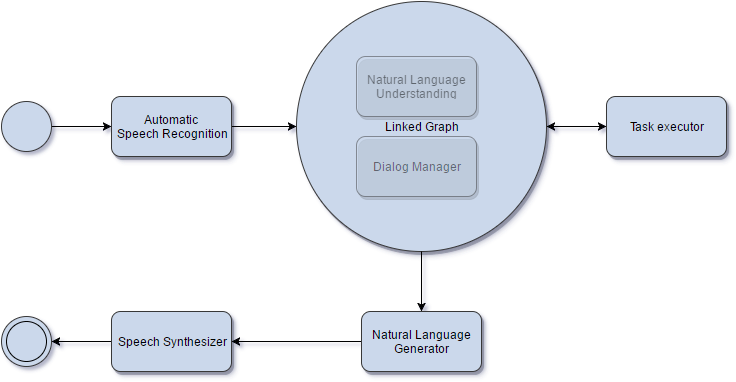
\includegraphics[width=\textwidth]{UsedArch}
\end{figure}

\subsection{Finite-State-Machine}

A finite state machine, better described on chapter 24 of \cite{speechlanguageprocessing}, is how user can navigate between possible tasks and is modeled as a linked graph. 
When user is in some state, knot, each one has it's own children linked via edge; each edge has two main 
properties; transition sentence and threshold. For each child transition sentence the Jaccard similarity
will be calculated with user input. The edge with the highest percentage that is greater than it's threshold
is going to make the graph navigate to linked child of the current knot. If none of the comparisons had
higher value than the threshold, the graph sends back an error message tha the navigation failed.

\begin{figure}[H]
    \caption[english]{Decision tree of the current graph}
    \centering
    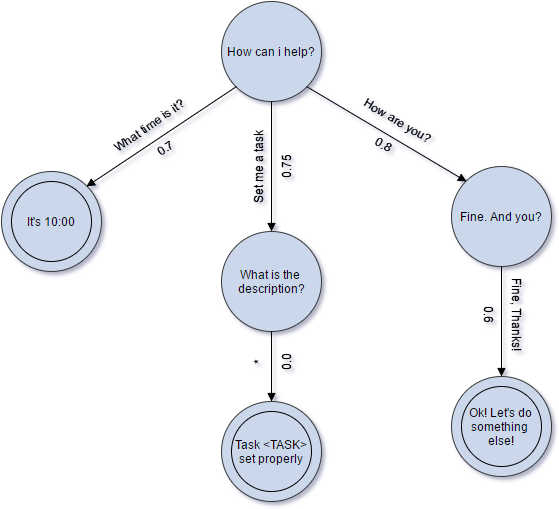
\includegraphics[width=\textwidth]{DecisionTree}
\end{figure}

\subsection{User Input Detection}

The most challenge obstacle is observed on watching the user audio input. Determining the valid interval
of audio buffer that represents an intended one is hard. Therefore, the system simplifies this task
creating an thirty seconds frame buffer and makes a constant scan looking for the frame slice that
starts with a pitch increase that is higher than a euristically pre defined threshold volume and ends
with pitch decrease that is lower than the same threshold.

\begin{figure}[H]
    \caption[english]{Detection of valid user input}
    \centering
    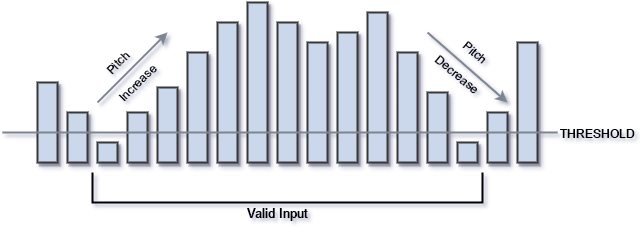
\includegraphics[width=\textwidth]{AudioBufferFrameSlice}
\end{figure}

\subsection{Pitch Detection}

Using vector dot product between last and current audio buffer slices we can detect if the pitch has
an increase or a decrease. These vectors are two dimensional; the x and y components are formed by
the frequency and the amplitude. The current vector uses the array at indexes one to its length
minus two, the previous vector uses the indexes zero and the length minus three and the next vector 
uses indexes two and length minus one and all of them uses the sabe buffer. If the dot product between 
the previous and the current vector is higher than the dot product between the current and the next
vector the pitch gets lower otherwise the pitch gets higher \cite{nonverbalvoiceinput}.

\begin{figure}[H]
    \caption[english]{Pitch detection}
    \centering
    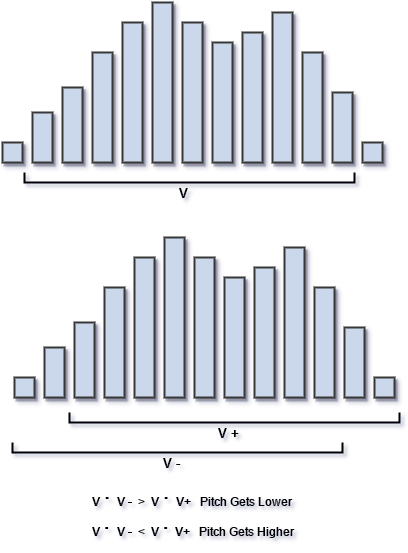
\includegraphics[width=0.5\textwidth]{PitchDetection}
\end{figure}

\section{Conclusion}

The system got working pretty well; the agent is correctly executing the pre defined tasks.
Some fixes may be required to voice detection to try to ignore noise and use a better valid
user input detection. The tasks may have an ordered way of execution to avoid confusion on
programming functions.

\medskip




\begin{thebibliography}{9}

\bibitem{nonverbalvoiceinput} 
Takeo Igarashi, John F. Hughes, 
\textit{Voice as Sound: Using Non-verbal Voice Input for Interactive Control}. 
Computer Science Department, Brown University 115 Waterman Street, Providence, R1 029912, USA.
 
\bibitem{speechlanguageprocessing} 
Daniel Jurafsky, James H. Martin, 
\textit{Speech and Language Processing, 2nd Edition}.
ISBN-13: 978-0131873216.
ISBN-10: 0131873210.
 
\bibitem{chatbots} 
Dan	Jurafsky, 
\\\texttt{http://web.stanford.edu/class/cs124/lec/chatbot.pdf},
Stanford University.

\end{thebibliography}
 
\end{document}
